\section{Decidability of the FO-Theory}\label{sec:decidability}
Recall that the Cayley-graph of the queue monoid $\Qx$ induced by $A$ is denoted by $\frakC=(\Qx,(E_\alpha)_{\alpha\in\Sigma})$.
In order to ease the notation we let elements of $\frakC$ inherit some properties from their projections to the read and write actions. 
For $p,q\in \Qx$ let $|p| = |(\rd{p}, \wrt{p})|$, $p\Delta q = (\rd{p}, \wrt{p})\Delta (\rd{q}, \wrt{q})$, and we call $|p\Delta q|$ the \emph{($\Delta$-)distance} of $p$ and $q$. Note that $\Delta$ defines a metric on $\frakC$. Further for $\vec{p} = (p_1,\ldots,p_k)\in \Qx^k$ let 
$\calN_r(\vec{p}) = \{ q\in \Qx \mid \exists 1\leq i \leq k\colon |p_i\Delta q| \leq r \vee |q| \leq r \}$ be the \emph{$(\Delta-)$neighborhood} of $\vec{p}$ of radius $r$ (\emph{$r$-neighborhood}). Note that we implicitly add the origin
of $\frakC$ to $\vec{p}$ when we compute the neighborhood. Moreover we define the notion of a border-decomposition and an $r$-skeleton for an element $p\in\Qx$ as the border-decomposition and the $r$-skeleton of $\rd{p} \sqcap \wrt{p}$.

Let us first give an intuitive outline of our decidability proof. We follow a classical proof strategy due to Ferrante and Rackoff \cite{FerR79}. Roughly speaking  we show that there is some fixed primitive recursive function $f:\bbN \to \bbN$ such that for every
two $({r+1})$-equivalent tuples $\vec{p},\vec{q} \in \Qx^n$ and every $p\in \Qx$ there is a $q$ in the $f(r+1)$-neighborhood of the tuple $\vec{q}$ such that $(\vec{p},p) \equiv_r (\vec{q}, q)$.
This implies that in order to evaluate a formula $Qx\phi(\vec{p})$ where $\phi$ has quantifier rank $r$ and $Q\in\{\exists,\forall\}$  we can restrict the quantification of $x$ to the $f(r+1)$-neighborhood of $\vec{p}$. Since the
$r$-neighborhood of each element $p\in \Qx$ is finite and effectively computable for every radius $r$, we can use the above observation to implement a decision procedure for the theory of $\frakC$.   
In order to achieve this goal we exploit the fact that first-order logic cannot measure distances between two nodes that are more than exponentially far away in the quantifier rank. Therefore our task for a given quantifier rank $r>0$ is to find for every $p$ that is far away from a tuple $\vec{p}$ an element $p'$ that is closer (but not yet too close) to $\vec{p}$ such that the neighborhoods of $p$ and $p'$ of a suitably chosen radius are not distinguishable with the remaining quantifier rank $r-1$. What makes this task more complex than for most other examples of Cayley-graphs with decidable first-order theory that can be found in the literature is that the Cayley-graph of the queue monoid is in some sense less local.
In fact, the neighborhood-structure of an element $p$ does not only depend on suffixes of  bounded length of $\rd{p}$ and $\wrt{p}$ (as it would be the case for instance for the direct product of two free monoids). We solve this problem via the notion of skeletons. Our proof 
reveals that   the $r$-type of the $2^{r+1}$-neighborhood of an element $p$ is basically determined by the $(r+1)$-type of the $3\cdot 2^{r+1}$-skeleton of $\rd{p} \sqcap \wrt{p}$. This will be the core
of our proof.

Let us start off by making some technical preparations in order to formulate the core idea precisely.
\begin{definition}
	Let $V$ be an $r$-skeleton. We say that $q\in\Qx$ is \emph{compatible} with $V$ 
	if $V$ has an instantiation $v$ such that $\rd{q} \sqcap \wrt{q}= vx$ for some $x\in A^{\leq r}$ and 
	$|\wrt{q} \Delta v| \leq r$.
\end{definition}
Intuitively, $q$ being compatible to an $r$-skeleton $V$ means that we can obtain an element
$q'$ with $r$-skeleton $V$ by deleting up to $r$ many read actions and modifying the write
actions arbitrarily up to distance $r$. We use this notion in order to translate elements of the Cayley-graph
into positions of an $r$-skeleton. Next we describe how we translate back and forth between elements of the Cayley-graph and positions in a skeleton.
However we can not guarantee that every element in close proximity to a given element $p$ can be associated with a position in the $r$-skeleton of $p$ because small changes to the read and write actions might change the border-decomposition dramatically. But we can modify
$r$ and $p$ slightly to circumvent this problem.  
\begin{definition}
	For $q\in\Qx$ with $|\rd{q}| \geq r$ let $\cpr_r(q)$ be the element $q'$  with $\wrt{q'} = \wrt{q}$, $\rd{q'}=\rd{q}\suf_{r}({\rd{q}})^{-1}$, and $\mu({q'}) = \rd{q'} \sqcap \wrt{q'}$.
	In other words, $\cpr_r$ just cuts the last $r$ read actions and pushes read and write actions as far together as possible. 
	%	\begin{center}
	%	\begin{tikzpicture}[scale=0.85,every node/.style={scale=0.85}]
	%	\path[draw, fill=red!10] (0,0) rectangle (5,0.25);
	%	\path[draw, fill=blue!10] (1.5, 0) rectangle (6.5, -.25);
	%	\draw[draw, decorate, decoration={brace,amplitude=5pt}] (2.5, .25) -- node[above, yshift= 5pt] {$r$} (5, .25);
	%	\node at (8, 0) {$\mapsto$};
	%	\path[draw, fill=red!10] (9.5,0) rectangle (12,0.25);
	%	\path[draw, fill=blue!10] (11, 0) rectangle (16, -.25);
	%	\draw[draw, decorate, decoration={brace,amplitude=5pt}] (12, .25) -- node[above, yshift= 5pt] {$r$} (14.5, .25);
	%	\path[draw, dotted] (12, 0) rectangle (14.5, .25);
	%	\end{tikzpicture}
	%	\end{center}
\end{definition}
\begin{definition}
	Let $p,q\in \Qx$ and let $U$ and $V$ be the $3r$-skeletons of $\cpr_{2r}(p)$ and $\cpr_{2r}(q)$, respectively. If we suppose that $(m_1,\ldots,m_k)$ are positions in $V$ and $(n_1,\ldots,n_k)$ are positions in $U$ such that $(U,m_1,\ldots,m_k) \equiv_{\ell} (V,n_1,\ldots,n_k)$ for some $\ell \geq 1$. For $p'\in \Qx$ with $|p'\Delta p| \leq r$ and $|\mu(p')| \geq 2r$ we associate a position $m_{k+1}$ in $U$ as follows:
	Let $(u_1,\ldots, u_m)$ be the complete border-decomposition of $\rd{\cpr_{2r}(p)}$ and $(v_1,\ldots,v_n)$ be the complete border-decomposition of $\rd{\cpr_{2r}(q)}$. As $p'$ has distance at most $r$ from $p$ we have that $\rd{p'} = \rd{\cpr_{2r}(p)}x$
	for some $x\in A^{\leq 2r}$. Therefore there is an $i\leq m$ such that $\mddl{p'} = u_ix$. Then $i$ is the position that is associated with $p'$.
	
	Now let $n_{k+1}$ be such that $(U,m_1,\ldots,m_{k+1}) \equiv_{\ell-1} (V,n_1,\ldots,n_{k+1})$ we associate an element $q'$ with $n_{k+1}$ as follows:
	Let $q'$ be the element with $\rd{q'} = \rd{\cpr_{2r}(q)}u_{m_{k+1}}^{-1}\mddl{p'}$, $\wrt{q'}\Delta\wrt{\cpr_r({q})} = \wrt{p'}\Delta\wrt{\cpr_{2r}({p})}$, and 
	$\mddl{q'} = v_{m_{k+1}}u_{n_{k+1}}^{-1}\mddl{p'}$. Note that $q'$ is well defined since $V[j]$ is labeled by $\pref_{2^{r+2}}(u_i^{-1}\mddl{p})$. Therefore $v_j\pref_{2^{r+1}}(v_i^{-1}\mddl{p})$ is a prefix of $\wrt{q'}$ by construction.
\end{definition}

Another important ingredient of our proof is to construct ``small'' $r$-equivalent words from a given word $w$. This is routine since it can be achieved by a simple automata-theoretic approach.
\begin{restatable}{mylem}{thomaszeug}[\!\!\cite{Tho97}]\label{lem:r-equiv_word_construction}
	From a given alphabet $\Gamma$, a word $v\in\Gamma^\ast$, and $r\in\bbN$ one can compute an automaton $\calA$ in time $\exp_{r+1}(f(r))$ with $L(\calA) = \{w\in \Gamma^\ast\mid w\equiv_r v \}$ for some primitive recursive function $f$.
\end{restatable}

We use this idea to  define a family of  equivalence relations $(\calE^r_m)_{r,m\in\bbN}$.
For $r,m\in \bbN$ and $\vec{p},\vec{q}\in \Qx^m$ let $\vec{p} \calE^r_m \vec{q}$ iff
\begin{bracketenumerate}
	\item If $|p_i \Delta \epsilon| \leq 4\exp_{r+2}(2, f(r))$ then $p_i=q_i$ where $f$ is the function from Lemma \ref{lem:r-equiv_word_construction}.
	\item\label{item:E_distance} $|p_i \Delta p_j| =_{2^r} |q_i\Delta q_j|$ for all $1\leq i, j\leq m$ and if $|p_i\Delta p_j| \leq 2^r$ then also $p_i \Delta p_j = q_i\Delta q_j$. 
	\item\label{item:E_partition} There is a partition $X_1,\ldots,X_k$ of $\{1,\ldots,m\}$ such that for $X\neq X'\in \{X_1,\ldots,X_k\}$ it holds that with $\text{min} = \min X$: 
	\begin{alphaenumerate}
		\item\label{item:part_distance} If $i\in X$, $j\in X'$ it holds that $|p_i\Delta p_j| > 2^r$ (and therefore $|q_i\Delta q_j| > 2^r$).
		\item\label{item:E_suffix} $\suf_{2^{r+m+2}}(\rd{p_i}) = \suf_{2^{r+m+2}}(\rd{q_i})$ and \\$\suf_{2^{r+m+2}}(\wrt{p_i}) = \suf_{2^{r+m+2}}(\wrt{q_i})$ for all $i\in X$.
		\item For all $j\in X$ it holds that $|p_\text{min} \Delta p_j| \leq \sum_{s= r}^{r+m} 2^s$ (and therefore also $|q_\text{min} \Delta q_j| \leq \sum_{s= r}^{r+m} 2^s$).
		\item\label{subitem:E_partition:equivalence} Let $U$ be the $3\cdot 2^{r+m+1}$-skeleton of $\cpr_{2^{r+m+2}}(p_\text{min})$ and $V$ be the $3\cdot 2^{r+m+1}$-skeleton $\cpr_{2^{r+m+2}}(q_\text{min})$. Then for all 
		$j\in X$ we have that either $\mu(p_j) = \mu(q_j)$ or $|\mu(p_j)| \geq 2^{r+m+2}$ and $p_j$ is compatible with $U$ and $q_j$ is compatible with $V$. Further if $m_1,\ldots, m_k$ are the positions in $U$ that are associated with $\{p_j \mid j\in X \}$ and $n_1,\ldots, n_k$ are the positions in $U$ that are associated with $\{q_j \mid j\in X \}$ then $(V,m_1,\ldots,m_k) \equiv_{r+1} (U,n_1,\ldots,n_k)$.
	\end{alphaenumerate}  
\end{bracketenumerate} 
We show that $(\calE^r_m)_{r,m\in\bbN}$ are indeed EF-relations for $\frakC$.
\begin{lemma}\label{lem:partial_isomorphism}
	For all $m\in\bbN_{>0}$ and all $\vec{p},\vec{q} \in \Qx^m$: If $\vec{p} \calE^0_m \vec{q}$ then the mapping $p_i \mapsto q_i$ is a partial isomorphism.
\end{lemma}
\begin{proof}
	We need to show that $(p_i,p_j)\in E_a \Rightarrow (q_i,q_j)\in E_a$  for all $i,j\leq m$ and all $a\in \Sigma$.
	Let $\vec{p}, \vec{q} \in \Qx^m$ with $\vec{p} \calE^0_m \vec{q}$. Suppose  $(p_i,p_j) \in E_a$ for some $a\in\Sigma$. Then $|p_i\Delta p_j| = 1$. Hence $p_i\Delta p_j = q_i\Delta q_j$ by (\ref{item:E_distance}). 
	Let $X_1,\ldots, X_k$ be the partition from Property \ref{item:E_partition}. Since the distance between $p_i$ and $p_j$ and between $q_i$ and $q_j$ is $1$ we derive from Property (\ref{item:part_distance}) that $i$ and $j$ belong to the same 
	$X\in\{X_1,\ldots, X_k\}$. Let $\ell = \min X$.
	If $|\mu(p_i)| < 2^{m  +2}$ then, by Property (\ref{subitem:E_partition:equivalence}) and (\ref{item:E_suffix}), $\mu(p_i) = \mu(q_i)$. In this case $(p_i, p_j) \in E_a \Leftrightarrow (q_i,q_j) \in E_a$  obviously holds.
	Otherwise there are $3\cdot2^{m + 1}$-skeletons $U,V$ such that 
	$p_i$ and $p_j$ can be translated into positions $m_1, m_2$ in $U$ and $q_i$ and $q_j$ can be translated into position $n_1,n_2$ in $V$ such that $(U,m_1,m_2) \equiv_1 (V,n_1,n_2)$. 
	There are two possible types of configurations for $p_i$ and $p_j$ such that they can be connected by an edge. First, it might be the case  that $\rd{p_i} = \rd{p_j}$,
	$\wrt{p_i}a = \wrt{p_j}$, and $\mddl{p_i} = \mddl{p_j}$. In this case $m_1=m_2$ and therefore $n_1=n_2$, which implies that $\rd{q_i} = \rd{q_j}$,
	$\wrt{q_i}a = \wrt{q_j}$, and $\mddl{q_i} = \mddl{q_j}$. Therefore $(q_i,q_j) \in E_a$.
	
	Second, it might be that $\rd{p_i}a = \rd{p_j}$ (where $a=\ov{b}$),
	$\wrt{p_i} = \wrt{p_j}$, and $\mddl{p_j}a^{-1}$ is the largest suffix $w$ of $\mddl{p_i}$ such that $wa$ is a prefix of $\wrt{p_i}$.  This property can be translated into the formula of quantifier rank $1$. Let $(w_0,\ldots, w_n)$ be the complete border-decomposition of $\cpr_{2^{m+2}}(p_\ell)$ and $v:= w_{m_1}^{-1}\mddl{p_i} \in A^{\leq 3\cdot 2^{m+1}}$. Then
	\[\phi(x_1, x_2) \coloneq x_2 \leq x_1 \land \bigvee_{s\in A^{\leq 3\cdot 2^{m+1}} : (va)\preceq s} P_s(x_2) \land  \forall y: \left(x_2 < y < x_1 \to \bigwedge_{s\in A^{\leq 3\cdot 2^{m+1}} : va\preceq s} \lnot P_s(y)\right) . \]
	 Hence $U \models \phi(m_1,m_2)$  and since $(U,m_1,m_2) \equiv_1 (V, n_1,n_2)$ also $V \models \phi(n_1, n_2)$ and therefore $(q_i,q_j)\in E_a$.
\end{proof}


\begin{lemma}\label{lem:EF_relations}
	For all $m,r\in\bbN$ and all $\vec{p},\vec{q}\in \Qx^m$:  
	\[\vec{p} \calE^{r+1}_m \vec{q} \Rightarrow \forall p\in \Qx \exists q\in \calN_{\exp_{r+3}(g(r+m))}(\vec{q}): (\vec{p}, p) \calE^{r}_{m+1} (\vec{q}, q)\]
	for some primitive recursive function $g$.
\end{lemma}
\begin{proof}
	Let $f$ be the primitive recursive function from Lemma \ref{lem:r-equiv_word_construction}.
	Let $\vec{p}, \vec{q} \in \Qx^m$ with $(\vec{p}, \vec{q}) \in \calE^{r+1}_m$ and 
	let $X_1,\ldots,X_k$ be a partition of $\{1,\ldots,m\}$ with the properties described in (\ref{item:E_partition}). 
	%Further let $X_i(\vec{p}) = \{p_j \mid j\in X_i \}$ and $X_i(\vec{q}) = \{q_j \mid j\in X_i \}$. 
	Consider $p\in \Qx$. We distinguish three cases.
	If $p$ has distance $\leq 4\exp_{r+2}(2, f(r))$ from $\epsilon$ then we choose $q=p$.
	
	From now on suppose $p$ has distance $> 4\exp_{r+2}(2, f(r))$ from $\epsilon$.
	We consider the case that $p$ has distance $>2^r$ from every $p_i$.
	Since the distance from $\epsilon$ is exactly $|\strt{p}| + 2|\mddl{p}| + |\rght{p}|$ it follows that $|\strt{p}| > \exp_{r+2}(f(r))$ or $|\mddl{p}| > \exp_{r+2}(f(r))$ or $|\rght{p}| > \exp_{r+2}(f(r))$. 
	%	 If $|\lambda(a)| > 2^r$ then we choose a $v\in \Sigma^\ast$ such that  
	%    $\rd{a}\suf_{2^{r}}(\rd{a})^{-1} \sqcap \wrt{a} = v\,\rd{a}\suf_{2^{r}}(v\,\rd{a})^{-1} \sqcap \wrt{b}$. If $x$ is the first letter of $\wrt{a}$ then we can choose $v= y^\ell$ for some $y\neq x$ and some $\ell\in\bbN$. 
	%    Let $b_\ell$ be the element with $\rd{b_\ell} = y^\ell \rd{a}$, $\wrt{b_\ell} = \wrt{a}$, and $\mu(b) = \mu(a)$.
	%    As there are only $m$ other elements chosen so far, we can choose $\ell$ large enough so that the element $b$ has distance $>2^{r}$ from every $b_i$ and from $\epsilon$. If   
%	Basically, we want to use the $3\cdot 2^{r+1}$-skeleton of $p$ to construct a suitable answer $q$. However, we need to cut the last $2^{r+1}$ read actions in order to avoid certain problems that would occur if we want to translate elements in close proximity to $p$ into positions of the $3\cdot 2^{r+1}$-skeleton.   
	Let $p'= \cpr_{2^{r+m+2}}(p)$.  Consider 
	the $3\cdot 2^{r+m+1}$-skeleton $V = \calS_{3\cdot 2^{r+m+1}}(p')$. By Lemma \ref{lem:r-equiv_word_construction} we can find a $3\cdot 2^{r+m+1}$-skeleton $W$ of length at most $(m+1)\exp_{r+2}(f(r+1))$ with $V \equiv_{r+1} W$ and $3\cdot 2^{r+m+1}$-instantiation $w$ with $|w|\leq  c\cdot 2^{(m+1)\exp_{r+2}(f(r+1)) \cdot 3\cdot 2^{r+m+1}}  \leq \exp_{r+3}(g(r+m))$ (for a suitable primitive recursive function $g$). Using Lemma \ref{lem:short_ends_construction}, words $u,v$ of length at most 
	$(m+1)2^{r+m+3}$ such that 
	\begin{enumerate}
		\item $\suf_{2^{r+m+2}}(uw) = \suf_{2^{r+m+2}}(\rd{p}\suf_{2^{r+m+2}}(\rd{p})^{-1} )$
		\item $\suf_{2^{r+m+2}}(wv) = \suf_{2^{r+m+2}}(\wrt{p})$
		\item $\pref_{2^{r+m+2}}(wv) = \pref_{2^{r+m+2}}(\wrt{p})$
		\item $uw\sqcap wv = w$
	\end{enumerate}
    such that every element $x$ with $\rd{x} = uw$ and $\wrt{x} = wv$ has distance $> 2^r$ from every $q_i$.
    We choose to $q$ to be such an element $x$. It remains to specify $\mddl{x}$. if $|\mddl{p}| \leq 2^{r+m+2}$ then choose $\mu(q) = \mu(p)$. Otherwise
	let $(v_0,v_1,\ldots, v_m)$ be the complete border-decomposition of $p'$ and let $(w_0, w_1,\ldots, w_n)$ be the complete border-decomposition of $w$. Let $i$
	be the index of $\mddl{p'}$ in $(v_0,v_1,\ldots, v_m)$. Because $\calS_{3\cdot 2^{r+m+1}}(p') \equiv_{r+1} W$ there is a $j\in \{0,\ldots,n\}$ such that $(\calS_{3\cdot 2^{r+m+1}}(p'), i) \equiv_r (W,j)$.
	Now choose $\mu(q) = w_j$. Finally extend the partition by $X_{k+1} = \{m+1\}$.
	
	%As the tuples $(\vec{a}, a)$ and $(\vec{a},b)$ fulfill the precondition of Lemma \ref{lem:EF_relations}, we can derive that the two tuples are $r$-equivalent. 
	
	If $p$ has distance $\leq 2^{r}$ from some $p_i$ then let $Y\in \{X_1,\ldots,X_k\}$ be such that $i\in Y$ and let $j=\min Y$. Let $U$ be the $3\cdot 2^{r+m+1}$-skeleton of $\cpr_{2^{r+m+2}}(p_j)$ and 
	$V$ be the $3\cdot 2^{r+m+1}$-skeleton of $\cpr_{2^{r+m+2}}(q_j)$.
	Since $|p_i\Delta p_j| \leq \sum_{s=r+1}^{r+m} 2^s$ and $|p\Delta p_i| \leq 2^r$ we conclude that $|p\Delta p_j| \leq \sum_{s=r}^{r+m} 2^s \leq 2^{r+m+1}$. Hence, $p$ is compatible with $U$. Let $m_1,\ldots,m_\ell$ be the positions in $U$ that are associated with the elements $\{q_s \mid s\in Y\}$, $m_{\ell+1}$ the position in $U$ that is associated with $p$, and $n_1,\ldots,n_\ell$ be the positions associated with $\{q_s \mid s\in Y\}$ in $V$. Since $(U,m_1,\ldots,m_\ell) \equiv_{r+2} (V,n_1,\ldots,n_\ell)$ by Property (\ref{subitem:E_partition:equivalence}) there exists a $n_{\ell+1}$ with $(U,m_1,\ldots,m_{\ell+1}) \equiv_{r+1} (V,n_1,\ldots,n_{\ell+1})$. From $n_{\ell+1}$ we compute the associated element $q$
	in the $(\sum_{s= r+m}^{r} 2^s)$-neighborhood of $q_j$.
	\begin{figure}[h]
		\centering\begin{center}
	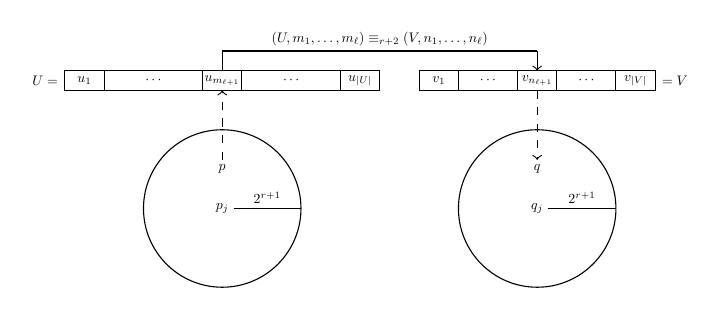
\begin{tikzpicture}[scale=0.5,every node/.style={scale=0.5}]
	 \draw (0,1) circle (2cm);
	 \draw (8,1) circle (2cm);
	 
	 \node (pj) at (0,1) {$p_j$};
	 \node (qj) at (8,1) {$q_j$};
	 \draw (pj) -- node[above] {$2^{r+1}$}  (2,1); 
	 \draw (qj) -- node[above] {$2^{r+1}$}  (10,1);
	 
	 \node (p) at (0, 2) {$p$};
	 \node (q) at (8, 2) {$q$};
	 
	 \path[draw] (-4, 4) rectangle (4,4.5);
	 \node at (-4.5, 4.25) {$U=$};
	 \draw (-3, 4) -- (-3, 4.5);
	 \draw (-.5, 4) -- (-.5, 4.5);
	 \draw (.5, 4) -- (.5, 4.5);
	 \draw (3, 4) -- (3, 4.5);
	 \node at (-3.5, 4.25) {$u_1$};
	 \node at (-1.75, 4.25) {$\cdots$};
	 \node at (0, 4.25) {$u_{m_{\ell + 1}}$};
	 \node at (1.75, 4.25) {$\cdots$};
	 \node at (3.5, 4.25) {$u_{|U|}$};
	 
	 \path[draw] (5, 4) rectangle (11,4.5);
	 \node at (11.5, 4.25) {$=V$};
	 \draw (6, 4) -- (6, 4.5);
	 \draw (7.5, 4) -- (7.5, 4.5);
	 \draw (8.5, 4) -- (8.5, 4.5);
	 \draw (10, 4) -- (10, 4.5);
	 \node at (5.5, 4.25) {$v_1$};
	 \node at (6.75, 4.25) {$\cdots$};
	 \node at (8, 4.25) {$v_{n_{\ell + 1}}$};
	 \node at (9.25, 4.25) {$\cdots$};
	 \node at (10.5, 4.25) {$v_{|V|}$};
	 
	 \draw[->, dashed] (p) -- (0, 4);
	 \draw[->, dashed] (8,4) -- (q);
	 
	 \path[draw] (0, 4.5) -- (0, 5) edge node[above] {$(U, m_1,\ldots, m_\ell) \equiv_{r+2} (V, n_1,\ldots,n_\ell)$} (8, 5) 
	                     (8, 5)            edge[->] (8, 4.5);
	              
	 
	\end{tikzpicture}
\end{center}
		\caption{\label{fig:construction}Construction of $q$ from $p$ using $U$ and $V$.}
	\end{figure}
	The construction of $q$ ensures that Properties (\ref{item:E_suffix}) to (\ref{item:E_partition}) are fulfilled for $(\vec{p}, p)$ and $(\vec{q}, q)$ by adding $\ell+1$ to $Y$. Hence $(\vec{p}, p) \calE^r_m (\vec{q}, q)$.
\end{proof}

The Lemmata \ref{lem:partial_isomorphism} and \ref{lem:EF_relations} ensure that $\calE^r_m$-equivalent tuples are also $r$-equivalent.

\begin{corollary}\label{cor:equivalence}
	For all $\vec{p}\in \Qx^m$, $p\in \Qx$, and $r\in\bbN$ there exists an element $q\in \calN_{\exp_{r+3}(g(r+m))}(\vec{p})$ with $(\frakC, \vec{p}, p) \equiv_r (\frakC,\vec{p}, q)$ for some polynomial~$f$.
\end{corollary}
%\begin{lemma}
%	There is a primitive-recursive function $f\colon \bbN \to \bbN$ such that for all $r\in\bbN_{>0}$, all $m$-tuples $\vec{a}\in C^m$, and all $a\in C$ there exists a $b \in \calN_{f(r)}(\vec{a})$ such that $(\calC, \vec{a}, a) \equiv_r (\calC, \vec{a}, b)$
%\end{lemma}
%\begin{proof}
%	Let $\vec{a}\in C^m$ and $a_{m+1} \in C$. If $a_{m+1}\in \calN_{2^{r+4}}(\vec{a})$ then we can choose $b_{m+1} = a_{m+1}$ and be done. Otherwise 
%	the tuple  
%	$\chi(a') = (\lambda(a'), \mu(a'), \rho(a'))$. Since $a$ has distance $> 2^{r+4}$ from the origin $\epsilon$ and 
%	$|\Delta(\epsilon, a_{m+1})| = |\lambda(a_{m+1})| + 2|\mu(a_{m+1})| + |\rho(a_{m+1})|$ it follows that at least one of the three values $|\theta(a_{m+1})|$,  $\theta\in \{\lambda,\mu, \rho \}$, is larger than $(2^{r+4} - 2^{r+1})/4  > 2^{r+2} - 2^{r+1} = 2^{r+1}$.  
%\end{proof}
%\begin{definition}
%	For $a\in C$  let $\cut_r(a) \in C$ be the element.  
%\end{definition}
As the size of the $r$-neighborhood of an element $p$ can be bounded by a primitive recursive function in $r$, $\rd{p}$, and $\wrt{p}$ we obtain our main result.
\begin{restatable}{mythm}{decidable}
	$\FOTh{\frakC}$ is primitive recursive.
\end{restatable}
